


\tikzset{every picture/.style={line width=0.75pt}} %set default line width to 0.75pt        

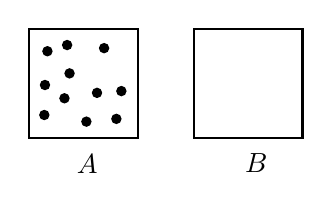
\begin{tikzpicture}[x=0.40,y=0.40,yscale=-1,xscale=1]
    %uncomment if require: \path (0,375); %set diagram left start at 0, and has height of 375

%Shape: Square [id:dp5886506825268709] 
\draw  [color={rgb, 255:red, 0; green, 0; blue, 0 }  ,draw opacity=1 ] (181,91.16) -- (279.34,91.16) -- (279.34,189.5) -- (181,189.5) -- cycle ;
%Shape: Square [id:dp24242986167867575] 
\draw   (330,91.16) -- (428.34,91.16) -- (428.34,189.5) -- (330,189.5) -- cycle ;
%Shape: Circle [id:dp48354636802020234] 
\draw  [fill={rgb, 255:red, 0; green, 0; blue, 0 }  ,fill opacity=1 ] (194.19,111.5) .. controls (194.19,109.46) and (195.85,107.8) .. (197.9,107.8) .. controls (199.94,107.8) and (201.6,109.46) .. (201.6,111.5) .. controls (201.6,113.55) and (199.94,115.21) .. (197.9,115.21) .. controls (195.85,115.21) and (194.19,113.55) .. (194.19,111.5) -- cycle ;
%Shape: Circle [id:dp8547166774432848] 
\draw  [fill={rgb, 255:red, 0; green, 0; blue, 0 }  ,fill opacity=1 ] (214.19,131.5) .. controls (214.19,129.46) and (215.85,127.8) .. (217.9,127.8) .. controls (219.94,127.8) and (221.6,129.46) .. (221.6,131.5) .. controls (221.6,133.55) and (219.94,135.21) .. (217.9,135.21) .. controls (215.85,135.21) and (214.19,133.55) .. (214.19,131.5) -- cycle ;
%Shape: Circle [id:dp3635316819967491] 
\draw  [fill={rgb, 255:red, 0; green, 0; blue, 0 }  ,fill opacity=1 ] (191.39,169.1) .. controls (191.39,167.06) and (193.05,165.4) .. (195.1,165.4) .. controls (197.14,165.4) and (198.8,167.06) .. (198.8,169.1) .. controls (198.8,171.15) and (197.14,172.81) .. (195.1,172.81) .. controls (193.05,172.81) and (191.39,171.15) .. (191.39,169.1) -- cycle ;
%Shape: Circle [id:dp504377272845598] 
\draw  [fill={rgb, 255:red, 0; green, 0; blue, 0 }  ,fill opacity=1 ] (245.39,108.7) .. controls (245.39,106.66) and (247.05,105) .. (249.1,105) .. controls (251.14,105) and (252.8,106.66) .. (252.8,108.7) .. controls (252.8,110.75) and (251.14,112.41) .. (249.1,112.41) .. controls (247.05,112.41) and (245.39,110.75) .. (245.39,108.7) -- cycle ;
%Shape: Circle [id:dp40762374287455616] 
\draw  [fill={rgb, 255:red, 0; green, 0; blue, 0 }  ,fill opacity=1 ] (229.39,175.1) .. controls (229.39,173.06) and (231.05,171.4) .. (233.1,171.4) .. controls (235.14,171.4) and (236.8,173.06) .. (236.8,175.1) .. controls (236.8,177.15) and (235.14,178.81) .. (233.1,178.81) .. controls (231.05,178.81) and (229.39,177.15) .. (229.39,175.1) -- cycle ;
%Shape: Circle [id:dp8577561818936912] 
\draw  [fill={rgb, 255:red, 0; green, 0; blue, 0 }  ,fill opacity=1 ] (260.99,147.5) .. controls (260.99,145.46) and (262.65,143.8) .. (264.7,143.8) .. controls (266.74,143.8) and (268.4,145.46) .. (268.4,147.5) .. controls (268.4,149.55) and (266.74,151.21) .. (264.7,151.21) .. controls (262.65,151.21) and (260.99,149.55) .. (260.99,147.5) -- cycle ;
%Shape: Circle [id:dp3598710056160941] 
\draw  [color={rgb, 255:red, 0; green, 0; blue, 0 }  ,draw opacity=1 ][fill={rgb, 255:red, 0; green, 0; blue, 0 }  ,fill opacity=1 ] (238.99,149.1) .. controls (238.99,147.06) and (240.65,145.4) .. (242.7,145.4) .. controls (244.74,145.4) and (246.4,147.06) .. (246.4,149.1) .. controls (246.4,151.15) and (244.74,152.81) .. (242.7,152.81) .. controls (240.65,152.81) and (238.99,151.15) .. (238.99,149.1) -- cycle ;
%Shape: Circle [id:dp8070234513651793] 
\draw  [fill={rgb, 255:red, 0; green, 0; blue, 0 }  ,fill opacity=1 ] (256.49,172.6) .. controls (256.49,170.56) and (258.15,168.9) .. (260.2,168.9) .. controls (262.24,168.9) and (263.9,170.56) .. (263.9,172.6) .. controls (263.9,174.65) and (262.24,176.31) .. (260.2,176.31) .. controls (258.15,176.31) and (256.49,174.65) .. (256.49,172.6) -- cycle ;
%Shape: Circle [id:dp3126762302018198] 
\draw  [fill={rgb, 255:red, 0; green, 0; blue, 0 }  ,fill opacity=1 ] (211.99,105.9) .. controls (211.99,103.86) and (213.65,102.2) .. (215.7,102.2) .. controls (217.74,102.2) and (219.4,103.86) .. (219.4,105.9) .. controls (219.4,107.95) and (217.74,109.61) .. (215.7,109.61) .. controls (213.65,109.61) and (211.99,107.95) .. (211.99,105.9) -- cycle ;
%Shape: Circle [id:dp24135298904714841] 
\draw  [fill={rgb, 255:red, 0; green, 0; blue, 0 }  ,fill opacity=1 ] (209.59,154) .. controls (209.59,151.96) and (211.25,150.3) .. (213.3,150.3) .. controls (215.34,150.3) and (217,151.96) .. (217,154) .. controls (217,156.05) and (215.34,157.71) .. (213.3,157.71) .. controls (211.25,157.71) and (209.59,156.05) .. (209.59,154) -- cycle ;
%Shape: Circle [id:dp9432634536780442] 
\draw  [fill={rgb, 255:red, 0; green, 0; blue, 0 }  ,fill opacity=1 ] (191.99,142) .. controls (191.99,139.96) and (193.65,138.3) .. (195.7,138.3) .. controls (197.74,138.3) and (199.4,139.96) .. (199.4,142) .. controls (199.4,144.05) and (197.74,145.71) .. (195.7,145.71) .. controls (193.65,145.71) and (191.99,144.05) .. (191.99,142) -- cycle ;

% Text Node
\draw (221.73,201.87) node [anchor=north west][inner sep=0.75pt]    {$\text{A}$};
% Text Node
\draw (373.8,201.54) node [anchor=north west][inner sep=0.75pt]    {$\text{B}$};


\end{tikzpicture}